\section{Approach} \label{sec:approach}
\begin{figure*}[t!]
\centering
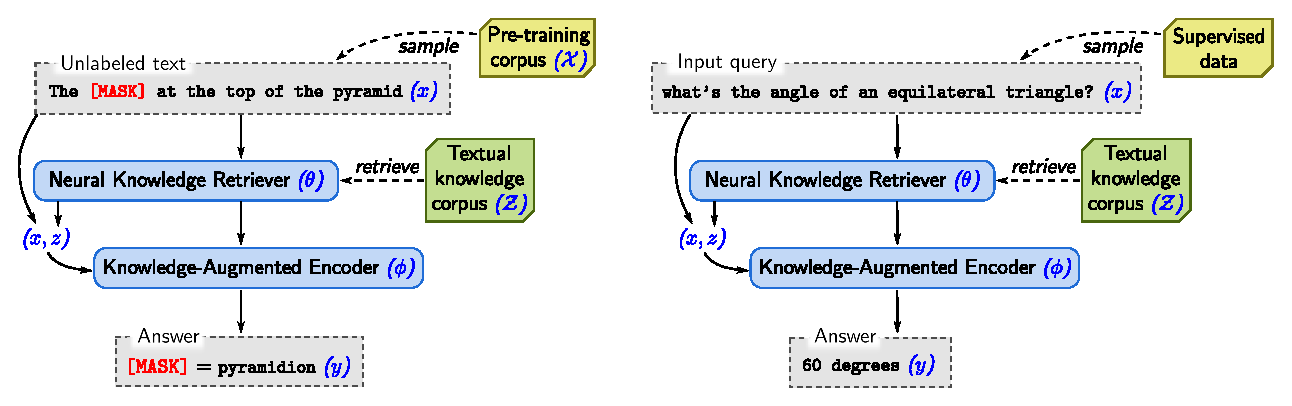
\includegraphics[width=.9\textwidth]{figures/pretrain_finetune.eps}
\caption{The overall framework of \thename. {\bf Left:} {\em Unsupervised pre-training.} The knowledge retriever and knowledge-augmented encoder are jointly pre-trained on the unsupervised language modeling task. 
{\bf Right:} {\em Supervised fine-tuning.} After the parameters of the retriever ($\theta$) and encoder ($\phi$) have been pre-trained, they are then fine-tuned on a task of primary interest, using supervised examples.}
\label{fig:approach}
\end{figure*}

% mini-intro; Overall structure;
We start by formalizing \thename's pre-training and fine-tuning tasks as a {\em retrieve-then-predict} generative process in Section~\ref{sec:generative_process}. Then in Section~\ref{sec:model_architecture}, we describe the model architectures for each component of that process. In Section~\ref{sec:training}, we show how to implement \thename pre-training and fine-tuning by maximizing the likelihood of \thename's generative process. En route, we address important computational challenges, explain why training works, and also discuss strategies for injecting useful inductive biases. The overall framework is illustrated in Figure~\ref{fig:approach}.
%, and we will refer to it throughout this section.

\subsection{\thename's generative process}
\label{sec:generative_process}
%
For both pre-training and fine-tuning, \thename takes some input $x$ and learns a distribution $p(y \mid x)$ over possible outputs $y$. %predicts an output $y$. As we will detail, \thename defines a probability distribution, $p(y \mid x)$.
For pre-training, the task is masked language modeling: $x$ is a sentence from a pre-training corpus $\cX$ with some tokens masked out, and the model must predict the value of those missing tokens, $y$. For fine-tuning, the task is \openqa: $x$ is a question, and $y$ is the answer.

\thename decomposes $p(y\mid x)$ into two steps: {\em retrieve}, then {\em predict}. Given an input $x$, we first retrieve possibly helpful documents $z$ from a knowledge corpus $\cZ$. We model this as a sample from the distribution $p(z\mid x)$. Then, we condition on both the retrieved $z$ and the original input $x$ to generate the output $y$---modeled as $p(y\mid z,x)$. To obtain the overall likelihood of generating $y$, we treat $z$ as a latent variable and marginalize over all possible documents $z$, yielding % the following overall likelihood for the entire generative process:
\begin{equation}
p(y \mid x) = \sum_{z \in \cZ} p(y \mid z, x)\, p(z \mid x). \label{eqn:marginal}
\end{equation}

\subsection{Model architecture}
\label{sec:model_architecture}
We now describe the two key components: % of the generative process in Equation~\ref{eqn:marginal}:
the \textbf{neural knowledge retriever}, which models $p(z\mid x)$, and the \textbf{knowledge-augmented encoder}, which models $p(y\mid z,x)$.

\paragraph{Knowledge Retriever}
%The retriever has the form:
The retriever is defined using a dense inner product model:
\begin{align*}
p(z \mid x) &= \frac{\exp{f(x, z)}}{\sum_{z'} \exp{f(x,z')}}, \\
f(x, z) &= \inputembed(x)^\top \docembed(z),
\end{align*}
where $\inputembed$ and $\docembed$ are embedding
functions that map $x$ and $z$ respectively to $d$-dimensional vectors.
%We refer to $f(x, z)$ as the ``relevance score'' between $x$ and $z$. This score is simply the inner product between the vector embeddings of $x$ and $z$.
The \emph{relevance score} $f(x, z)$ between $x$ and $z$ is defined as the inner product of the vector embeddings.
The retrieval distribution is the softmax over all relevance scores.

We implement the embedding functions using BERT-style Transformers \cite{bert}. Following standard practices, we join spans of text by applying wordpiece tokenization, separating them with $\sep$ tokens, prefixing a $\cls$ token, and appending a final $\sep$ token.
\begin{align*}
    \joinbert(x) & = \cls x \sep \\
    \joinbert(x_1, x_2) & = \cls x_1 \sep x_2 \sep
\end{align*}
As in \citet{bert}, we pass this into a Transformer, which produces one vector for each token, including the vector corresponding to $\cls$ which is used as a ``pooled'' representation of the sequence (denoted $\bertsub{CLS}$). Finally, we perform a linear projection to reduce the dimensionality of the vector, denoted as a projection matrix $\mathbf{W}$:%. All together, we have,
\begin{align*}
\inputembed(x) & = \mathbf{W_\mathtt{input}}\bertsub{CLS}(\joinbert(x)) \\
\docembed(z) & = \mathbf{W_\mathtt{doc}}\bertsub{CLS}(\joinbert(z_\text{title}, z_\text{body}))
\end{align*}
where $z_\text{title}$ is the document's title and $z_\text{body}$ is its body.
%If the knowledge corpus doesn't have document titles, we can just use the body text.
We let $\theta$ denote all parameters associated with the retriever, which include the Transformer and projection matrices.

\paragraph{Knowledge-Augmented Encoder}
Given an input $x$ and a retrieved document $z$, the knowledge-augmented encoder defines $p(y\mid z,x)$. We join $x$ and $z$ into a single sequence that we feed into a Transformer (distinct from the one used in the retriever). This allows us to perform rich cross-attention between $x$ and $z$ before predicting $y$. See Figure~\ref{fig:intro} for a concrete example.

At this stage, the architectures for pre-training and fine-tuning differ slightly. For the masked language model pre-training task, we must predict the original value of each \mask token in $x$. To do so, we use the same masked language modeling (MLM) loss as in \citet{bert}:
\begin{align*}
\centering
p(y\mid z,x) &= \prod_{j=1}^{J_x} p(y_j \mid z, x) \\
p(y_j \mid z, x) &\propto \exp \left(w_j^\top \bert_{\mathtt{MASK}(j)}(\joinbert(x, z_\text{body}))\right)
\end{align*}
where $\bert_{\mathtt{MASK}(j)}$ denotes the Transformer output vector corresponding to the $j^{th}$ masked token, $J_x$ is the total number of \mask tokens in $x$, and $w_j$ is a learned word embedding for token $y_j$.

For \openqa fine-tuning, we wish to produce the answer string $y$. Following previous reading comprehension work \cite{squad,bidaf,rasor,bidaf_plusplus}, we will assume that the answer $y$ can be found as a contiguous sequence of tokens in some document $z$.
%Since we have already selected a document $z$ using the retriever, the encoder simply needs to select a contiguous span from $z$ to be its prediction for $y$.
Let $S(z, y)$ be the set of spans matching $y$ in $z$. Then we can define $p(y \mid z,x)$ as:
\begin{align*}
p(y \mid z, x)  &\propto \sum_{s \in S(z, y)} \exp\left(\mathtt{MLP}\left(\left[h_{\mathtt{START(s)}} ; h_{\mathtt{END(s)}}\right]\right)\right)\\
h_{\mathtt{START(s)}} &= \bertsub{START(s)}(\joinbert(x, z_\text{body})), \\
h_{\mathtt{END(s)}} &= \bertsub{END(s)}(\joinbert(x, z_\text{body})),
\end{align*}
where $\bertsub{START(s)}$ and $\bertsub{END(s)}$ denote the Transformer output vectors corresponding to the start and end tokens of span $s$, respectively, while $\mathtt{MLP}$ denotes a feed-forward neural network. We will let $\phi$ denote all parameters associated with the knowledge-augmented encoder.

\subsection{Training}
\label{sec:training}

For both pre-training and fine-tuning, we train by maximizing the log-likelihood $\log p(y\mid x)$ of the correct output $y$. Since both the knowledge retriever and knowledge-augmented encoder are differentiable neural networks, we can compute the gradient of $\log p(y\mid x)$ (defined in Equation~\ref{eqn:marginal}) with respect to the model parameters $\theta$ and $\phi$, and optimize using stochastic gradient descent.

The key computational challenge is that the marginal probability
$p(y\mid x) = \sum_{z \in \cZ} p(y\mid x,z)\,p(z \mid x)$
involves a summation over all documents $z$ in the knowledge corpus $\cZ$. We approximate this by instead summing over the top $k$ documents with highest probability under $p(z \mid x)$---this is reasonable if most documents have near zero probability.

Even with this approximation, we still need an efficient way to find the top $k$ documents. %, as the naive method involves computing $p(z \mid x)$ for all $z$.
Note that the ordering of documents under $p(z \mid  x)$ is the same as under the relevance score $f(x, z) = \inputembed(x)^\top \docembed(z)$, which is an inner product. Thus, we can employ Maximum Inner Product Search (MIPS) algorithms to find the approximate top $k$ documents, using running time and storage space that scale sub-linearly with the number of documents \cite{mips_cone,mips_alsh,mips_binary}.

To employ MIPS, we must pre-compute $\docembed(z)$ for every $z \in \cZ$  and construct an efficient search index over these embeddings. However, this data structure will no longer be consistent with $p(z \mid x)$ if the parameters $\theta$ of $\docembed$ are later updated. Hence, the search index goes ``stale'' after every gradient update on $\theta$.

Our solution is to ``refresh'' the index by asynchronously re-embedding and re-indexing all documents every several hundred training steps. The MIPS index is slightly stale between refreshes, but note that it is {\em only} used to select the top $k$ documents. We recompute $p(z \mid x)$ and its gradient, using the fresh $\theta$, for these top $k$ documents after retrieving them.
In Section~\ref{sec:ablation}, we empirically demonstrate that this procedure results in stable optimization, provided that refreshes happen at a sufficiently frequent rate.

\paragraph{Implementing asynchronous MIPS refreshes}
We asynchronously refresh the MIPS index by running two jobs in parallel: a primary {\em trainer} job, which performs gradient updates on the parameters, and a secondary {\em index builder} job, which embeds and indexes the documents. As shown below, the trainer sends the index builder a snapshot of its parameters, $\theta'$. The trainer then continues to train while the index builder uses $\theta'$ to construct a new index in the background. As soon as the index builder is done, it sends the new index back to the trainer, and the process repeats.

{
\begin{figure}
\begin{center}
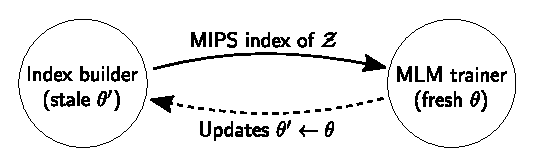
\includegraphics[width=.8\columnwidth]{figures/trainer_generator.eps}
\caption{\thename pre-training with asynchronous MIPS refreshes.}
\end{center}
\end{figure}
}

While asynchronous refreshes can be used for both pre-training and fine-tuning, in our experiments we only use it for pre-training. For fine-tuning, we just build the MIPS index once (using the pre-trained $\theta$) for simplicity and do not update $\docembed$.\footnote{This works because pre-training already yields a good $\docembed$ function. However, it is possible that refreshing the index would further improve performance.} Note that we still fine-tune $\inputembed$, so the retrieval function is still updated from the query side.

\paragraph{What does the retriever learn?}
Since the knowledge retrieval of \thename is latent, it is not obvious how the training objective encourages meaningful retrievals. Here, we show how it rewards retrievals that improve prediction accuracy.

For a given query $x$ and document $z$, recall that $f(x,z)$
is the ``relevance score'' that the knowledge retriever assigns to document $z$.
We can see how a single step of gradient descent during \thename pre-training alters this score by analyzing
the gradient with respect to the parameters of the knowledge retriever, $\theta$:
\begin{align*}
\nabla \log p(y \mid x) & =\sum_{z\in\cZ} r(z) \nabla f(x,z) \\
r(z) & =\left[\frac{p(y \mid z,x)}{p(y \mid x)}-1\right]p(z \mid x).
\end{align*}
For each document $z$, the gradient encourages
the retriever to change the score $f(x,z)$ by $r(z)$ --- 
increasing if $r(z)$ is positive, and decreasing if negative.
The multiplier $r(z)$
is positive if and only if $p(y\mid z,x) > p(y\mid x)$.
The term $p(y\mid z,x)$ is the probability of predicting
the correct output $y$ when using document $z$.
The term $p(y \mid x)$ is the expected value of $p(y \mid x, z)$ when randomly sampling a document from $p(z \mid x)$. Hence, document $z$ receives a positive update whenever it performs better than expected.
%\footnote{In Appendix B, we further show that when a single document provides ``all'' the value, \thename resembles supervised learning.}

\subsection{Injecting inductive biases into pre-training} \label{sec:inductive-bias}
In the process of developing \thename, we discovered several additional strategies that further guide the model towards meaningful retrievals, described below.

\paragraph{Salient span masking}
During \thename pre-training, we want to focus on examples $x$ that require world knowledge to predict the masked tokens. As explained in Section~\ref{sec:background}, some MLM spans only require local context. To focus on problems that require world knowledge, we mask \emph{salient spans} such as \nl{United Kingdom} or \nl{July 1969}. We use a BERT-based tagger trained on CoNLL-2003 data \cite{conll_ner} to identify named entities, and a regular expression to identify dates. We select and mask one of these salient spans within a sentence for the masked language modeling task. We show that this significantly outperforms other masking strategies in Section~\ref{sec:ablation}.

\paragraph{Null document}
Even with salient span masking, not all masked tokens require world knowledge to predict. We model this by adding an empty \emph{null document} $\znull$~to the top $k$ retrieved documents, allowing appropriate credit to be assigned to a consistent sink when no retrieval is necessary.

\paragraph{Prohibiting trivial retrievals}
If the pre-training corpus $\cX$ and the knowledge corpus $\cZ$ are the same, there exists a trivial retrieval candidate $z$ that is \emph{too} informative: if the masked sentence $x$ comes from document $z$, the knowledge augmented encoder can trivially predict $y$ by looking at the unmasked version of $x$ in $z$. This results in a large positive gradient for $p(z\mid x)$. If this occurs too often, the knowledge retriever ends up learning to look for exact string matches between $x$ and $z$, which does not capture other forms of relevance. For this reason, we exclude this trivial candidate during pre-training.

\paragraph{Initialization}
At the beginning of training, if the retriever does not have good embeddings for $\inputembed(x)$ and $\docembed(z)$, the retrieved documents $z$ will likely be unrelated to $x$. This causes the knowledge augmented encoder to learn to ignore the retrieved documents. Once this occurs, the knowledge retriever does not receive a meaningful gradient and cannot improve, creating a vicious cycle. To avoid this cold-start problem, we warm-start $\inputembed$ and $\docembed$ using a simple training objective known as the Inverse Cloze Task (ICT) where, given a sentence, the model is trained to retrieve the document where that sentence came from. We defer to ~\citet{orqa} for details. For the knowledge-augmented encoder, we warm-start it with BERT pre-training---specifically, the uncased BERT-base model (12 layers, 768 hidden units, 12 attention heads).
